% Gemini theme
% See: https://rev.cs.uchicago.edu/k4rtik/gemini-uccs
% A fork of https://github.com/anishathalye/gemini

\documentclass[final]{beamer}

% ====================
% Packages
% ====================
\usepackage{amsfonts}
\usepackage[T1]{fontenc}
\usepackage{lmodern}
\usepackage[dvipsnames,table,xcdraw]{xcolor}
\usepackage{array}
\usepackage[size=custom,width=120,height=72,scale=1.0]{beamerposter}
\geometry{paperwidth=42in,paperheight=32.5in}
\usetheme{gemini}

\definecolor{UBCblue}{rgb}{0.04706, 0.03725, 0.76667} 
\usecolortheme{wolverine}

\usepackage{graphicx}
\usepackage{booktabs}
\usepackage{subfig}
\usepackage{qrcode}
\usepackage{graphicx}
\usepackage{subcaption}
\usepackage[ruled,vlined]{algorithm2e}
% \bibliographystyle{unsrtnat}
\usepackage{mathtools}
\usepackage{wrapfig}
\usepackage{multirow}
\usepackage{textcomp}
% \usepackage{MnSymbol,wasysym}
\usepackage{wasysym}
\usepackage{tikzsymbols}
\usepackage{parskip}
%\usepackage{enumitem}
\usepackage{makecell}
\usepackage{caption}
\usepackage{float}
\usepackage{subcaption}
\usepackage{lineno}


\usepackage{tikz}
\usepackage{pgfplots}
\pgfplotsset{compat=1.17}
\usepackage{tcolorbox}
\tcbuselibrary{theorems}

\newtcbtheorem{mytheo}{}{colback=white!5}{th}
 
 

% ====================
% Lengths
% ====================

% If you have N columns, choose \sepwidth and \colwidth such that
% (N+1)*\sepwidth + N*\colwidth = \paperwidth
\newlength{\sepwidth}
\newlength{\colwidth}
\setlength{\sepwidth}{0.025\paperwidth}
\setlength{\colwidth}{0.3\paperwidth}
\definecolor{ForestGreen}{RGB}{34,139,34}
\definecolor{LimeGreen}{rgb}{0.2, 0.8, 0.2}
\newcommand{\separatorcolumn}{\begin{column}{\sepwidth}\end{column}}

% ====================
% Title
% ====================

\title{Kantorovich Strikes Back! Wasserstein GANs are not Optimal Transport?}

\author{Korotin Alexander \inst{\star,1,2}, \and Kolesov Alexander  \inst{\star,2} \quad \& \and Burnaev Evgeny \inst{1,2}}

\institute[shortinst]{\inst{1} \textit{ Skolkovo Institute of Science and Technology },\quad \inst{2} \textit{ Artificial Intelligence Research Institute (AIRI)} ,\\[0.7 cm] \inst{\star} \textit{  Equal contribution }
}


% ====================
% Footer (optional)
% ====================


% (can be left out to remove footer)

% ====================
% Logo (optional)
% ====================

% use this to include logos on the left and/or right side of the header:
% \logoright{\includegraphics[height=7cm]{logo1.pdf}}
% \logoleft{\includegraphics[height=7cm]{logo2.pdf}}

% ====================
% Body
% ====================

\begin{document}
\addtobeamertemplate{headline}{}
{
    \begin{tikzpicture}[remember picture,overlay]
      \node [anchor=north west, inner sep=3cm] at ([xshift=0.0cm,yshift=2.9cm]current page.north west)
      {\includegraphics[width=12.0cm]{logos/skolog.jpeg}}; % also try shield-white.eps
      \node [anchor=north est, inner sep=3cm] at ([xshift=0.0cm,yshift=38.7cm]current page.north est)
      {\includegraphics[width=12.0cm]{logos/airilogo.jpeg}};
       
    \end{tikzpicture}
    \noindent\rule{\textwidth}{1pt}
}
 

\begin{frame}[t]
\begin{columns}[t]
\separatorcolumn

\begin{column}{\colwidth}
\vspace{2 mm}
\noindent\fbox{
    \parbox{0.98\textwidth}{%
        \centering{\textbf{Question :}} How precisely do WGANs solve the OT problem?
    }%
}
\begin{alertblock}{\noindent\fcolorbox{black}{gray!25}{
    \parbox{0.98\textwidth}{%
        \centering{Background on Optimal Transport} .
    }}}
 For distributions $\mathbb{P},\mathbb{Q}$ on $\mathbb{R}^{D}$ the Monge's form of the Wasserstein-1 distance is
  $$ \mathbb{W}_{1}(\mathbb{P},\mathbb{Q}) = \min_{T \sharp \mathbb{P} = \mathbb{Q}}\int ||x - T(x)||_{2}d\mathbb{P}(x).$$
  The Kantorovich's relaxation is given by
  $$ \mathbb{W}_{1}(\mathbb{P},\mathbb{Q})= \min_{\pi \in \Pi(\mathbb{P},\mathbb{Q})}\int_{\mathbb{R}^{D} \times \mathbb{R}^{D}} || x - y ||_{2}d\pi(x,y).$$
  \begin{figure}
      \centering
      \includegraphics[width = 30cm]{logos/monge.png}
      \caption{Monge's and Kantorovich's OT formulations.}
      \label{fig:my_label}
  \end{figure}
  \vspace{-9 mm}
  \end{alertblock}
  
  \begin{block}{ \noindent\fcolorbox{black}{gray!25}{
    \parbox{0.98\textwidth}{%
        \centering{\color{black}{Dual formulation of $\mathbb{W}_{1}$}} .
    }} }
    
For distributions $\mathbb{P},\mathbb{Q}$, the dual formulation of $\mathbb{W}_{1}$ is given by
  \begin{itemize}
  \item{ Conventional ($\lfloor \textbf{LS}\rceil$):
  $$ \mathbb{W}_{1}(\mathbb{P},\mathbb{Q}) = \max_{f \oplus g  \leq ||\cdot||_{2}}\int f(x)d\mathbb{P}(x) + \int g(y)d\mathbb{Q}(y);$$}
  \item{c-transform ($\lfloor \textbf{MM:B}\rceil$, $\lfloor \textbf{MM:Bv2}\rceil$, $\lfloor \textbf{MM}\rceil$, $\lfloor \textbf{MM:R}\rceil$):
  $$ \mathbb{W}_{1}(\mathbb{P},\mathbb{Q}) = \max_{f}\int f(x)d\mathbb{P}(x) + \int \min_{x \in \mathbb{R}^{D}} \{||x - y||_{2} - f(x)\} d\mathbb{Q}(y);$$}
  \item{ 1-Lipschitz constraint ($\lfloor \textbf{WC}\rceil$, $\lfloor \textbf{GP}\rceil$, $\lfloor \textbf{LP}\rceil$, $\lfloor \textbf{SN}\rceil$, $\lfloor \textbf{SO}\rceil$):
  $$ \mathbb{W}_{1}(\mathbb{P},\mathbb{Q}) = \max_{||f||_{L} \leq 1}\int f(x)d\mathbb{P}(x) - \int f(y)d\mathbb{Q}(y).$$}
  \end{itemize}
  Typically, the dual potential is recovered with neural nets which are trained with SGD.
  \end{block}

%=============================================%
 \begin{block}{ \noindent\fcolorbox{black}{gray!25}{
    \parbox{0.98\textwidth}{%
        \centering{\color{black}{Optimal Transport in GANs}} .
    }}}
 
Let $\mathbb{P} = \mathbb{P}_{\alpha}$ is a parametric distribution and $\mathbb{Q}$ is the data distribution. Typically, $ \mathbb{P}_{\alpha} = G_{\alpha}\sharp \mathbb{S}$ obtained by a generator network $G_{\alpha}$ from a fixed latent $\mathbb{S}$.\\[0.8 cm]
The \textbf{loss} function for the generator $G_{\alpha}$ is
\vspace{2 mm}
$$ \mathbb{W}_{1}(\mathbb{P}_{\alpha},\mathbb{Q}) = \int_{z} f^{*}(G_{\alpha}(z))d\mathbb{S}(z) - \int f^{*}(y)d\mathbb{Q}(y).$$
The derivative of the loss is
\vspace{4 mm} 
$$  \frac{\partial \mathbb{W}_{1}(\mathbb{P}_{\alpha},\mathbb{Q})}{\partial \alpha } = \int_{z} J_{\alpha}G_{\alpha}(z)^{T}\nabla f^{*}(G_{\alpha}(z))d\mathbb{S}(z).$$

\begin{figure}
\vspace{-1 cm}
\includegraphics[width=0.5\linewidth,scale=0.01]{logos/gan.png}
\vspace{-7 mm}
 \caption{ \centering The anti-gradient $-\nabla f^{*}(x)$ shows where to move the mass of each $x=G_{\alpha}(z)$ to make the generated $\mathbb{P}_{\alpha}$ closer to $\mathbb{Q}$ in $\mathbb{W}_{1}$.}
\end{figure}
\noindent\fbox{
    \parbox{0.98\textwidth}{%
        \centering{\textbf{Problem:}} There are no non-trivial pairs $\mathbb{P},\mathbb{Q}$ with known OT gradient $\nabla f^{*}$.
    }%
}
\end{block}
 

\end{column}

\separatorcolumn

\begin{column}{\colwidth}
%=================================================%   
\begin{block}{ \noindent\fcolorbox{black}{gray!25}{
    \parbox{0.98\textwidth}{%
        \centering{\color{black}{Constructing benchmark pairs.}}
    }}}

We propose a way to construct pairs of $\mathbb{P},\mathbb{Q}$ with a known OT map, cost, gradient.

\noindent\begin{minipage}{0.55\textwidth}%
\vspace{-10 mm}
\begin{mytheo}{Definition}{}
For a $1$-Lipschitz function $u:\mathbb{R}^{D}\rightarrow\mathbb{R}$, we say that a transport plan $\pi\in\Pi(\mathbb{P},\mathbb{Q})$ is $u$-\textit{ray monotone} (decreasing) if $u(x)-u(y)=\|x-y\|_{2}$ holds $\pi$-almost surely for $x,y\in\mathbb{R}^{D}.$
\end{mytheo} 
\vspace{8 mm}
\begin{mytheo}{Proposition}{}
    Let $\pi\in\Pi(\mathbb{P},\mathbb{Q})$ be a $u$-ray monotone transport plan for a $1$-Lipschitz function $u$. Then it is an optimal plan between $\mathbb{P},\mathbb{Q}.$
\end{mytheo} 

\end{minipage}%
\hfill%
\begin{minipage}
{0.45\textwidth}\RaggedRight
\begin{figure}
\vspace{1 mm}
\includegraphics[width=0.8\linewidth,scale=0.4]{logos/rays.png}
\vspace{-4 mm}
\caption{\centering Truncated transport rays of a random MinFunnel $N=16, D=2$.}
\end{figure}
\end{minipage}  
  
  
\vspace{-4 mm}\centering\textbf{Parameterizing 1-Lipschitz functions:}\\[0.5 cm]
$u:\mathbb{R}^{D}\rightarrow\mathbb{R}$, we employ the following $1$-Lipschitz \textit{MinFunnel} functions
$$u(x) =\min_{n} \left\lbrace \|x-a_{n}\|_{2}+b_{n}\right\rbrace.$$
\begin{figure}
      \centering
      \vspace{-9 mm}
      \includegraphics[width = 30cm]{logos/teaser.png}
      \caption{The pipeline of constructing of benchmark pairs.}
      \label{fig:teaser}
      \vspace{-4 mm}
  \end{figure}   
\centering\textbf{The construction pipeline:}
\centering
\begin{itemize}
    \item{Pick absolutely continuous distribution $\mathbb{P}$.}
    \item{Take 1-Lipschitz MinFunnel function $u(x)$.}
    \item{Find $u$'s transport rays, $u$-forward map.}
    \item{Move samples from $\mathbb{P}$ to   $\mathbb{Q}$ by the  map.}
\end{itemize}

 
 
 

 
 
 \end{block}
%======================================================%
\begin{block}{\noindent\fcolorbox{black}{gray!25}{
    \parbox{0.98\textwidth}{%
        \centering{\color{black}{High-dimensional and images benchmark pairs.}}
    }}}

\begin{figure}[!htb]
\minipage{0.49\textwidth}
  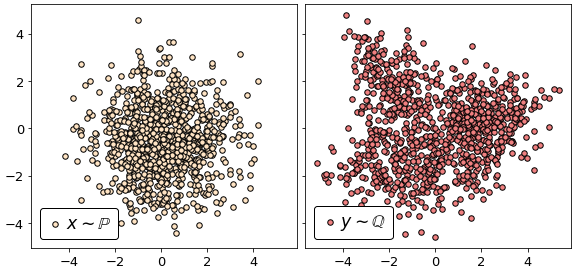
\includegraphics[width=\linewidth]{logos/pca_32d_4.png}
  \caption{\centering The pair with $N=4, D=32$.}
\endminipage\hfill
\minipage{0.49\textwidth}
  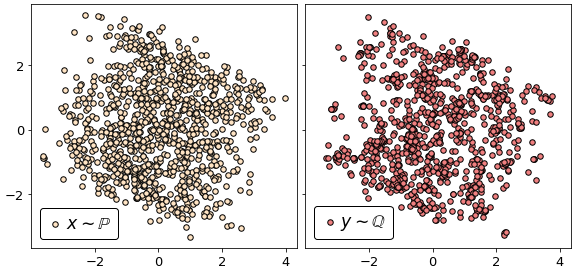
\includegraphics[width=\linewidth]{logos/pca_4d_64.png}
  \caption{\centering The pair with $N=64, D=4$.}
\endminipage


\end{figure}

\begin{figure}[!htb]
\minipage{0.49\textwidth}
  \includegraphics[width=\linewidth]{logos/celeba_1.png}
  \caption{\centering Samples of CelebA from the pair with $(N,p)=(1,10)$.}
\endminipage\hfill
\minipage{0.49\textwidth}
  \includegraphics[width=\linewidth]{logos/cifar_1.png}
  \caption{\centering Samples of CIFRA-10 from the pair with $(N,p)=(1,10)$.}
\endminipage


\end{figure}   
\begin{figure}[!htb]
\minipage{0.49\textwidth}
  \includegraphics[width=\linewidth]{logos/celeba_16.png}
  \caption{\centering Samples of CelebA from the pair with $(N,p)=(16,100)$.}
\endminipage\hfill
\minipage{0.49\textwidth}
  \includegraphics[width=\linewidth]{logos/cifar16.png}
  \caption{\centering Samples of CIFAR-10 from the pair with $(N,p)=(16,100)$.}
\endminipage


\end{figure} 
\end{block}


\end{column}

%-------------------third_column--------------------%
\separatorcolumn
\begin{column}{\colwidth}

\begin{block}{\noindent\fcolorbox{black}{gray!25}{
    \parbox{0.98\textwidth}{%
        \centering{\color{black}{Evaluating dual surfaces in 2D.}}
    }}}
 \begin{figure}
\subfloat[\centering $\lfloor \textbf{WC}\rceil$.]{\includegraphics[width=0.205\linewidth]{logos/surfaces_wc.png}}\hfill
\subfloat[\centering $\lfloor \textbf{GP}\rceil$.]{\includegraphics[width=0.19\linewidth]{logos/surfaces_gp.png}}\hfill
\subfloat[\centering $\lfloor \textbf{LP}\rceil$.]{\includegraphics[width=0.19\linewidth]{logos/surfaces_lp.png}}\hfill
\subfloat[\centering $\lfloor \textbf{SN}\rceil$.]{\includegraphics[width=0.19\linewidth]{logos/surfaces_sn.png}}\hfill
\subfloat[\centering $\lfloor \textbf{SO}\rceil$.]{\includegraphics[width=0.19\linewidth]{logos/surfaces_so.png}}\skip

\subfloat[\centering $\lfloor \textbf{LS}\rceil$.]{\includegraphics[width=0.205\linewidth]{logos/surfaces_ls.png}}\hfill
\subfloat[\centering $\lfloor \textbf{MM:B}\rceil$.]{\includegraphics[width=0.19\linewidth]{logos/surfaces_qp.png}}\hfill
\subfloat[\centering $\lfloor \textbf{MM:Bv2}\rceil$.]{\includegraphics[width=0.19\linewidth]{logos/surfaces_cowgan.png}}\hfill
\subfloat[\centering $\lfloor \textbf{MM}\rceil$.]{\includegraphics[width=0.19\linewidth]{logos/surfaces_mm.png}}\hfill
\subfloat[\centering $\lfloor \textbf{MM:R}\rceil$.]{\includegraphics[width=0.19\linewidth]{logos/surfaces_mmr.png}}
\caption{\centering Surfaces of potentials $f_{\theta}$ learned by OT solvers on the pair with $D=2, N=4$.
\protect\linebreak The ground truth optimal potential is in Figure \ref{fig:teaser}.}
\end{figure}
\vspace{-4 mm}
\end{block}

%=========================================================%
\begin{block}{\noindent\fcolorbox{black}{gray!25}{
    \parbox{0.98\textwidth}{%
        \centering{\color{black}{Qualitative comparison of dual solvers.}}
    }}}
    
\noindent\begin{minipage}{0.6\textwidth}%
  \begin{itemize}
      \item $\mathcal{L}^2$ - metric:
      $$\mathcal{L}^{2}(\nabla \hat{f},\nabla f^{*}) = ||\nabla{\hat{f}} - \nabla{f^{*}}||_{2}^{2}; $$
      \item Cosine similarity:
      $$ \cos(\nabla \hat{f},\nabla f^{*}) = \frac{\langle \nabla \hat{f},\nabla f^{*} \rangle}{||\nabla \hat{f}||_{2} ||\nabla f^{*}||_{2}};$$
      \item  Deviation of $ {\mathbb{\hat{W}}_{1}}$ from $\mathbb{W}_{1}$:\vspace{1 mm}
      $$\text{dev} = 100\%\cdot \frac{|\mathbb{W}_{1}-\widehat{\mathbb{W}}_{1}|}{\mathbb{W}_{1}} .$$
  \end{itemize}
\end{minipage}%
\hfill%
\begin{minipage}
{0.4\textwidth}\RaggedRight
\includegraphics[width=0.9\linewidth,scale=0.5]{logos/metrics_def.png}
\end{minipage}
\end{block}
%=======================================================%

\begin{block}{\noindent\fcolorbox{black}{gray!25}{
    \parbox{0.98\textwidth}{%
        \centering{\color{black}{Results.}}
    }}}

\begin{table} 
\begin{subtable}{\linewidth}
\begin{tabular}{|c|c|c|c|c|c|c|c|c|c|c|}
\hline
 &                   $\lfloor \textbf{WC}\rceil$ &                  $\lfloor \textbf{GP}\rceil$ &                  $\lfloor \textbf{LP}\rceil$ &              $\lfloor \textbf{SN}\rceil$  & $\lfloor \textbf{SO}\rceil$  & $\lfloor \textbf{LS}\rceil$ & $\lfloor \textbf{MM:B}\rceil$ &  $\lfloor \textbf{MM:Bv2}\rceil$ & $\lfloor \textbf{MM}\rceil$ & $\lfloor \textbf{MM:R}\rceil$      \\ \hline
\bf{HD} &\color{red}0.11 & \color{LimeGreen}0.56 &\color{LimeGreen}0.56 & \color{red}0.09 & \color{LimeGreen}0.61 & \color{red}-0.51 & \color{red}-0.54 & \color{orange}0.45& \color{LimeGreen}0.53& \color{orange}0.31  \\ \hline
 \bf{Img} &\color{orange}0.33 & \color{ForestGreen}0.92 &\color{ForestGreen}0.92 & \color{orange}0.35 &  - & \color{orange}0.36 & \color{orange}0.38 & \color{red}0.09& \color{orange}0.46& \color{ForestGreen}0.91  \\ \hline
\end{tabular}
 \caption{\centering{The top row demonstrates $cos$ for dual solvers for pairs with $N=256, D=128$, while the bottom row shows $cos$ for image pairs $N = 16, p = 100$}}
\end{subtable}

\begin{subtable}{\linewidth}
\centering
\begin{tabular}{|c|c|c|c|c|c|c|c|c|c|c|}
\hline
 &                   $\lfloor \textbf{WC}\rceil$ &                  $\lfloor \textbf{GP}\rceil$ &                  $\lfloor \textbf{LP}\rceil$ &              $\lfloor \textbf{SN}\rceil$  & $\lfloor \textbf{SO}\rceil$  & $\lfloor \textbf{LS}\rceil$ & $\lfloor \textbf{MM:B}\rceil$ &  $\lfloor \textbf{MM:Bv2}\rceil$ & $\lfloor \textbf{MM}\rceil$ & $\lfloor \textbf{MM:R}\rceil$      \\ \hline
\bf{HD} &\color{red}$\gg$10  & \color{orange}0.89 &\color{orange}0.9 & \color{red}1.57 & \color{orange}0.77 & \color{red}2.07 & \color{red}1.98 & \color{red}$\gg$10& \color{orange}0.73& \color{red}1.38  \\ \hline
 \bf{Img} & \color{red}$\gg$10  & \color{red}1.34 &\color{orange}1.12 & \color{red}3.32 &  - & \color{red}1.87 & \color{red}1.28 &  \color{red}$\gg$10 & \color{ForestGreen}0.16& \color{orange}0.95  \\ \hline
\end{tabular}
\caption{\centering{The top row demonstrates $\matchal{L}^{2}$ metric for dual solvers for pairs with $N=256, D=128$, while the bottom row shows $\mathcal{L}^{2}$ metric for image pairs $N = 16, p = 100$}}
\end{subtable}
\begin{subtable}{\linewidth}
\centering
\begin{tabular}{|c|c|c|c|c|c|c|c|c|c|c|}
\hline
 &                   $\lfloor \textbf{WC}\rceil$ &                  $\lfloor \textbf{GP}\rceil$ &                  $\lfloor \textbf{LP}\rceil$ &              $\lfloor \textbf{SN}\rceil$  & $\lfloor \textbf{SO}\rceil$  & $\lfloor \textbf{LS}\rceil$ & $\lfloor \textbf{MM:B}\rceil$ &  $\lfloor \textbf{MM:Bv2}\rceil$ & $\lfloor \textbf{MM}\rceil$ & $\lfloor \textbf{MM:R}\rceil$      \\ \hline
\bf{HD} &\color{red}0.36 & \color{orange}0.67 &\color{orange}0.69 & \color{red}0.12 & \color{orange}0.8 & \color{red}-0.32 & \color{red}-0.32 & \color{red}2.61& \color{orange}0.79& \color{LimeGreen}1.02  \\ \hline
 \bf{Img} &\color{red}$\gg$100 & \color{red}36.16 &\color{red}36.75 & \color{LimeGreen}13.26 &  - & \color{red}5.24 & \color{red}4.21 &\color{LimeGreen}24.36& \color{red}$\gg$100& \color{LimeGreen}23.46& \hline
\end{tabular}
\caption{\centering{The top row demonstrates $dev$ metric for dual solvers for pairs with $N=64, D=128$, while the bottom row shows $dev$ for image pairs $N = 16, p = 100$}}
\end{subtable}
\end{table}
\vspace{-5 mm}
\end{block}

\begin{block}{\noindent\fcolorbox{black}{gray!25}{
    \parbox{0.98\textwidth}{%
        \centering{\color{black}{Conclusion.}}
    }}}
\begin{itemize}
    \item{All the solvers should \textbf{not} be considered as \bf{meaningful estimators} of $\mathbb{W}_{1}$.}
    \item{The gradient $\nabla \hat{f}$ recovered by some solvers shows \textbf{positive} $cos$ with the ground-truth gradient $\nabla f^{*}$, but mostly they provide \textbf{poor} $\mathcal{L}^{2}$ metric.}
\end{itemize}

\vspace{6 mm}
\centering{More details and code are represented in GitHub page}.\\[0.4 cm] 
\vspace{-0.5mm}\includegraphics[width=0.17\linewidth,center]{logos/github_logo.png}

\vspace{-4mm}{\color{blue}\url{https://github.com/justkolesov/Wasserstein1Benchmark}}
\vspace{4 mm}

 
  \end{block}

\end{column}

\separatorcolumn
\end{columns}

\end{frame}

\end{document}
